\subsection{Grenzwerte von Zahlenfolgen}
\paragraph{Def. 1:} \parskp
Es sei $n_0 \in \mathbb{N}$. Eine Funktion $f$ mit $Db(f)=\{u\in \mathbb{N}|n\geq n_0\}$ und $Wb(f) \subset \mathbb{R}$ heißt reelle Zahlenfolge.\\
Schreibweise: \\
$a_n=f(n)$ \qquad ($n \in Db(f)$)\\
$\left(a_n\right)_{n\geq n_0}=\left(a_{n_0}, a_{n_0+1}, a_{n_0+2}, ...\right)$\\
oft $n_0=0$ oder $n_0=1$.
\subparagraph{Bsp. 1:} 
\begin{enumerate}[label=\alph*.)]
\item $a_n=(-1)^n\cdot n \quad (n \in \mathbb{N})\\
(a_n)=(0,-1,2,-3,4,...)$
\item $a_0=-1,\; a_n=n\cdot a_{n-1} \quad (n \in \mathbb{N}^*)$ \quad (rekursive Def.)\\
$(a_n)=(-1,-1,-2,-6,-24,...), \; a_n = -n!$
\item $a_n=\frac{3}{10}+\frac{3}{10^2}+...+\frac{3}{10^n} \quad (n\in \mathbb{N}^*)$\\
$(a_n)=(0.3, 0.33, 0.333, ... )$
\item $a_n=1+(-1)^n\frac{1}{n^2} \quad (n \in \mathbb{N}^*)$\\
$(a_n)=\left( \frac{5}{4}, \frac{8}{9}, \frac{17}{16}, \frac{24}{25},...\right)$
\end{enumerate}
\paragraph{Def. 2:} 
\begin{itemize}
\item $(a_n)$ heißt \emph{konvergent}, wenn es eine Zahl $a \in \mathbb{R}$ gibt mit folgender Eigenschaft:\\
Zu jedem $\varepsilon > 0$ existiert eine natürliche Zahl $n_0(\varepsilon)$, sodass für alle $n \geq n_0(\varepsilon)$ gilt: $|a_n-a|< \varepsilon$.
\item Die Zahl $a$ heißt \emph{Grenzwert} von $(a_n)$.\\
Schreibweisen:\\
$\boxed{a=\lim_{n\rightarrow \infty}(a_n)}$ oder $\boxed{a_n \underset{\color{gray}n\rightarrow\infty}{\longrightarrow} a}$
\item $(a_n)$ heißt \emph{divergent}, falls $(a_n)$ nicht konvergent ist.
\end{itemize}
\subparagraph{Diskussion}
\begin{enumerate}
\item Für $\varepsilon>0$ heißt $U_{\varepsilon}(a):=(a-\varepsilon, a+\varepsilon)$ (offenes Intervall) \emph{$\varepsilon$-Umgebung von $a$}.\\
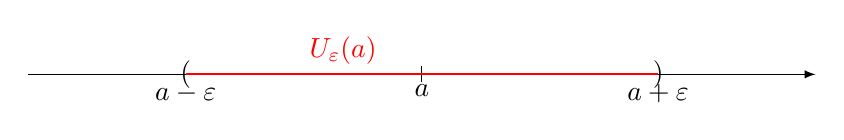
\begin{tikzpicture}
\draw [-latex] (-5,0) -- (5,0);
\draw (-3,0) node{(};
\draw (-3,0) node[below]{$a-\varepsilon$};
\draw (3,0) node{)};
\draw (3,0) node[below]{$a+\varepsilon$};
\draw (0,0.1) -- (0,-0.1);
\draw (0,0) node[below] {$a$};
\draw [red, thick] (-3,0)--(3,0);
\draw [red] (-1,0) node [above] {$U_{\varepsilon}(a)$};
\end{tikzpicture}\\
$\left( \lim_{n\rightarrow \infty}a_n=a\right)\equiv \left( \forall\varepsilon>0 \; \exists n_0(\varepsilon) \; \forall n\geq n_0(\varepsilon) \; a_n \in U_{\varepsilon}(a)\right)$\\
d.h. für jedes (noch so kleine) $\varepsilon$, liegen ab einem bestimmten (von $\varepsilon$ abhängigen) Index $n_0(\varepsilon)$ alle Glieder $a_n(n\geq n_0(\varepsilon))$ in $U_{\varepsilon}(a)$.
\item Im Bsp. 1 sind:\\
konvergente Folgen: \\
c.) mit $\underset{n\rightarrow\infty}{a_n}=\frac{1}{3}$\\
d.) mit $\underset{n\rightarrow\infty}{a_n}=1$\\
divergente Folgen: a.) und b.)
\item Ist $\underset{n\rightarrow\infty}{a_n}=0$, so heißt $(a_n)$ \emph{Nullfolge}.
\end{enumerate}
\paragraph{Def. 3:} \parskp
$(a_n)$ heißt:
\begin{itemize}
\item \emph{streng monoton wachsend}, falls für jedes $n$ gilt: $a_n<a_{n+1}$.
\item \emph{monoton wachsend}, falls für jedes $n$ gilt: $a_n\leq a_{n+1}$.
\item \emph{streng monoton fallend}, falls für jedes $n$ gilt: $a_n>a_{n+1}$.
\item \emph{monoton fallend}, falls für jedes $n$ gilt: $a_n\geq a_{n+1}$.
\end{itemize}
\paragraph{Def. 4:} \parskp
$(a_n)$ heißt beschränkt, wenn es eine Konstante $C>0$ gibt mit $|a_n|\leq C$ für alle $n$.
\subparagraph{Diskussion:}
\begin{enumerate}
\item $(a_n)$ beschränkt \\
$\Leftrightarrow \exists c>0 \; \forall n \quad |a_n| \leq C \\
\Leftrightarrow \exists c_1\in \mathbb{R}\; \exists c_2 \in \mathbb{R}\; \forall n \quad c_1 \leq a_n \leq c_2$
\item Folgen aus Bsp. 1:\\
\begin{tabular}{l l l l}
&Folge & Monotonie & Beschränktheit\\
a.)& $a_n=(-1)^n\cdot n$ & --  & --\\
b.)& $a_n=-n!$ & streng monoton fallend (ab $n=1$) & --\\
c.)& $a_n=\tfrac{3}{10}+\tfrac{3}{10^2}+...+\tfrac{3}{10^n}$ & streng monoton wachsend & $0,3\leq a_n < \tfrac{1}{3}$\\
d.) & $a_n=1+(-1)^n\tfrac{1}{n^2}$ & -- & $0\leq a_n <\tfrac{5}{4}$
\end{tabular}
\end{enumerate}
\paragraph{Satz 1:} \parskp
Jede konvergente folge ist beschränkt.
\paragraph{Satz 2:} \parskp
Jede monotone und beschränkte Folge ist konvergent.
\paragraph{Def. 5:} \parskp
$(a_n)$ heißt \emph{bestimmt konvergent} gegen $\begin{cases}
+\infty\\
- \infty
\end{cases}$, falls gilt: $\forall c \in \mathbb{R} \; \exists n_0(c) \; \forall n \geq n_0(c) \begin{cases}
a_n>c\\
a_n<c
\end{cases}$.\\
Schreibweise: $\boxed{\lim_{n\to \infty} a_n = \begin{cases}
+\infty\\
- \infty
\end{cases}}$
\subparagraph{Bsp. 2:} 
\begin{enumerate}[label=\alph*.)]
\item aus Bsp. 1c.): $a_n=\frac{3}{10}+...+\frac{3}{10^n}, \; (a_n)$ monoton wachsend und beschränkt $\Rightarrow (a_n)$ ist konvergent, $\lim_{n\to \infty}a_n = \frac{1}{3}$. 
\item aus Bsp. 1b.): $a_n=-n!$, $(a_n)$ monoton fallend und unbeschränkt $\Rightarrow$ $(a_n)$ ist bestimmt divergent, $\lim_{n\to \infty}a_n=-\infty$
\end{enumerate}
\subparagraph{Diskussion:}\parskp
Eine divergente Folge, die nicht bestimmt divergent ist, heißt \emph{unbestimmt divergent}.\\
Bpsw. Folge aus Bsp. 1a.) $a_n=(-1)^n\cdot n$.\bigskip\\
Einige wichtige Grenzwerte:
\begin{enumerate} [label=\alph*.)]
\item $\lim_{n\to \infty} \left(1+\frac{1}{n}\right)^n=e=2.71...$ (EULERsche Zahl)
\item $\lim_{n\to\infty} \sqrt[n]{n}=1$
\item $\lim_{n\to\infty} \frac{\ln n}{n}=0$
\item $\lim_{n \to \infty} \sqrt[n]{a}=1 \quad (a>0)$
\end{enumerate}
\paragraph{Satz 4:} Rechenregeln (Grenzwertsätze)\\
$(a_n)$ und $(b_n)$ seien zwei konvergente Folgen mit $\lim_{n\to \infty}=a, \; \lim_{n\to \infty} = b$. Dann gilt:
\begin{itemize}
\item $\lim_{n\to \infty}(a_n+b_n)=a+b$
\item $\lim_{n\to \infty}(c\cdot a_n)=c \cdot a$
\item $\lim_{n\to\infty} (a_n \cdot b_n) = a \cdot b$
\item $\lim_{n \to \infty} \left(\frac{a_n}{b_n}\right) = \frac{a}{b} \qquad (b_n\not = 0, b\not = 0)$
\end{itemize}
\subparagraph{Bsp. 3:}
\begin{enumerate} [label=\alph*.)]
\item $a_n=\frac{2n^2-1}{3n^2+n} \qquad (n=1,2,3,...)$\\
$a_n=\frac{n^2\left(2-\frac{1}{n^2}\right)}{n^2\left(3+\frac{n}{n^2}\right)}=\frac{2-\frac{1}{n^2}}{3+\frac{1}{n}}=\frac{\lim_{n\to\infty}\left(2-\frac{1}{n^2}\right)}{\lim_{n\to\infty}\left(3+\frac{1}{n}\right)}=\resultul{\frac{2}{3}}$\\
\fbox{Ausklammern der höchsten Potenzen in Zähler und Nenner}
\item $a_n=n\cdot \left(\sqrt{n^2+1}-n\right)$ \\
(in Klammern: „$\infty-\infty$“ $\curvearrowright$ Erweitern mit 3. binomischer Formel)\\
$a_n=\frac{n\cdot \left( \sqrt{n^2+1}-n\right) \cdot \tgreen{\left(\sqrt{n^2+1}+n\right)}}{\tgreen{\left(\sqrt{n^2+1}+n\right)}}
=\frac{n\cdot (n^2+1-n^2)}{n\cdot \sqrt{1+\frac{1}{n^2}}+n}
=\frac{n\cdot 1 }{n\left(\sqrt{1+\frac{1}{n^2}}+1\right)}
\underset{n\to \infty}{\longrightarrow} \frac{1}{2}$ \\
oder:
$\lim_{n\to\infty} = \resultul{\frac{ 1}{2}}$
\item $a_n=\frac{\sin n}{n} \qquad \left(0\leq |a_n|=\frac{|\sin n|}{n}\leq \frac{1}{n}\right)\Rightarrow\lim_{n\to\infty}a_n=0$\bigskip\\
Allgemein: $(a_n)$ beschränkt und $(b_n)$ bestimmt divergent $\Rightarrow\lim_{n\to\infty}\frac{a_n}{b_n}=0$.
\end{enumerate}

\subsection{Lineare Rekursionsgleichungen (Differenzengleichungen)}
\begin{itemize}
\item Allgemeine Form einer Rekursionsgleichung $k$-ter Ordnung:\\
$x_n=f(n,x_{n-1},x_{n-2},...,x_{n-k}) \qquad (k \geq 1,\; n\geq n_0+k)$
\item Wir betrachten nur \emph{lineare Rekursionsgleichungen mit konstanten Koeffizienten} (d.h. $a_j$ nicht von $n$ abhängig):\\
$\boxed{x_n=a_1 x_{n-1}+a_2 x_{n-2}+...+a_k a_{n-k}+h_n}\quad k\geq 1, \; a_k \not = 0, \; n\geq n_0 +k$\\
$x_n$ gesucht, $a_1,a_2,...,a_k, h_n \; (n\geq n_0)$ bekannt.
\item Indexverschiebung möglich:\\
$\boxed{x_{n+k}=a_1 x_{n+k-1}+a_2 x_{n+k-2}+...+a_k a_{n}+h_{n+k}}\quad (n\leq n_0)$\\
Wichtig ist die Differenz zwischen höchstem und niedrigstem Index von $x$ (=Ordnung der Rekursionsgleichung).
\item Da die größen $x_n, x_{n-1}, x_{n-2},...$ auch durch $x_n$ und die Differenzen $\Delta x_n:=x_n-x_{n-1}, \Delta^2x_n:=\Delta x_n-\Delta x_{n-1}=x_n-2x_{n-1}+x_{n-2}, ...$ ausgedrückt werden können, ist der Name \emph{Differenzengleichung} sehr verbreitet.
\item Die Differenzengleichung (aus erstem Punkt) heißt homogen, falls $h_n=0$ (für alle $n$), sonst inhomogen.
\end{itemize}
Zur Lösung von der Differenzengleichung (aus erstem Punkt oberhalb):
\begin{enumerate}
\item Allgemeine Lösung: $\boxed{x_n=x_n^{(h)}+x_n^{(p)}}$, dabei ist $x_n^{(h)}$ die \emph{allgemeine Lösung der zugehörigen homogenen Gleichung} $\boxed{x_n=a_1 x_{n-1}+...+a_k x_{n-k}}$ und $x_n^{(p)}$ eine \emph{partikuläre (spezielle) Lösung der inhomogenen Gleichung}.
\item Es gibt $k$ Lösungen $x_n^{(1)},...,x_n^{(h)}$ der homogenen Gleichung, so dass gilt:\\
$x_n^{(h)}=c_1 x_n^{(1)}+...+c_k x_n^{(h)}$\\
Diese erhält man mit Hilfe der Lösungen der charakteristischen Gleichung:\\
$\lambda^k=a_1 \lambda^{k-1}+a_2 \lambda^{k-2}+...+a_{k-1} \lambda+a_k$\\
Dise ergibt sich aus dem Ansatz:\\
$x_n^{(h)}= \lambda^n \; (\lambda \not = 0)\\
\Rightarrow \lambda^n = a_1 \lambda^{n-1}+...+a_k \lambda^{n-k} \quad |: \lambda^{n-k}\\
\Rightarrow $ Bei $k$ verschieden Lösungen $\lambda_1, ..., \lambda_2$ ergibt sich $x_n^{(h)}=c_1 \lambda_1^n+...+c_k \lambda_k^n$, falls z.B. $\lambda$ 2-fach auftritt, dann: $x_n^{(h)}=c_1\lambda_1^n+c_2\lambda_1^n\cdot n +...$
\item Für die Partikulärlösung $x_n^{(p)}$ führen spezielle Ansätze zum Ziel:\\
\begin{tabular}{ 
p{\dimexpr0.25\columnwidth-2\tabcolsep-1.5\arrayrulewidth} | >{\raggedright}
p{\dimexpr0.2\columnwidth-2\tabcolsep-1.5\arrayrulewidth} | >{\raggedright}
p{\dimexpr0.4\columnwidth-2\tabcolsep-1.5\arrayrulewidth}}
Inhomogenität $h_n$ & Bedingung & Ansatz für $x_n^{(p)}$\tabularnewline
\hline
Polynom in $n$ (Grad $r$) & $\lambda = 1$ ist keine$^{*)}$ Lösung von $\lambda^k$ & Polynom vom gleichen Grade mit unbestimmten Koeffizienten\tabularnewline
\hline
Potenzfunktion $b^n$ & $\lambda = b$ ist keine$^{*)}$ Lösung von $\lambda^k$ & $x_n^{(p)}=A \cdot b^n$
\end{tabular}\\
$^{*)}$ bei $\xi$-facher Lösung ist der Ansatz mit $n^\xi$ zu multiplizieren\\
Unbestimmte Koeffizienten $A, ...$ durch Einsetzen in die inhomogene Gleichung und Koeffizientenvergleich ermitteln.
\item Die $k$ Koeffizienten $c_1,...,c_k$ in der allgemeinen Lösung können durch die Anfangsbedingungen $(AB)$ (Vorgabe der ersten $k$ Glieder von $(x_n)$) ermittelt werden.\\
Es sind also folgende Schritte durchzuführen:
\begin{enumerate}[label=\Alph*)]
\item Allgemeine Lösung $x_n^{(h)}$ der homogenen Gleichung ermitteln
\item eine spezielle Lösung $x_n^{(p)}$ der inhomogenen Gleichung ermitteln
\item $x_n = x_n^{(h)}+x_n^{(p)}$
\item $AB$ erfüllen
\end{enumerate}
\end{enumerate}
\subparagraph{Bsp. 4:} $x_{n+1}=2 x_n +3 \qquad n\geq 0, \; x_0 =1$\\
Erste Glieder: $1,\; 5,\; 13,\; 29, ...$\\
Typ: Lineare Differenzengleichung 1. Ordnung\\
Lösung:
\begin{enumerate}[label=\Alph*)]
\item homogene Gleichung $x_{n+1}=2x_n$ (charakteristische Gleichung $\lambda_1 =2$)\\
$\lambda_1 =2 \; \Rightarrow \; x_n^{(h)}=C\cdot 2^n$
\item $h_n=3$ (Polynom des $0$-ten Grades). Ansatz: $x_n^{(p)}=A$ (Einsetzen in Ausgangsgleichung)\\
$A=2\cdot 2A+3 \; \Rightarrow \; A=-3 \;\Rightarrow\; x_n^{(p)}=-3$
\item $x_n = x_n^{(h)}+x_n^{(p)}=C\cdot 2^n-3$
\item $AB$: $n=0 \; \Rightarrow \; x_0 = 1 = C \cdot 2^0 \; \Rightarrow \; C=4$
\end{enumerate}
Also: $x_n=4 \cdot 2^n -3$
\subparagraph{Bsp. 5:} $x_{n+2}=x_{n+1}+2x_n \qquad n\geq 0, \; x_0 =2, \;x_1=3$\\
Erste Glieder: $2,\; 3, \; 7, \; 13,\; 27,\; 53, ...$\\
Typ: lineare homogene Dz.-Gleichung 2. Ordnung
\begin{enumerate}
\item[A)] Schritt A liefert bereits die allgemeine Lösung (B und C entfallen):
$\lambda^2=\lambda+2 \;\Rightarrow\; \lambda_1 = -1, \; \lambda_2 =2$\\
$\Rightarrow\; x_n=x_n^{(h)}=C_1 \cdot (-1)^n + C_2\cdot 2^n$
\item[D)] $AB$ erfüllen:\\
$C=\frac{5}{3},  \; C_1=\frac{1}{3} \begin{cases}
n=0 \; &\Rightarrow \; x_0 =2 = C_1+C_2\\
n=1 \; &\Rightarrow \; x_1 =3 = -C_1+2C_2
\end{cases}$
\end{enumerate}
Also: $x_n=\frac{1}{3}(-1)^n+\frac{5}{3}\cdot 2^n$
\subparagraph{Diskussion:} Bei einer homogenen linearen Dz.-Gleichung 2. Ordnung können folgende Fälle auftreten:
\begin{itemize}
\item $\lambda_1, \; \lambda_2$ reel und verschieden:\\
$\Rightarrow x_n = x_n^{(h)}= C_1 \lambda_1^n+C_2 \lambda_2^n$ (vgl. Bsp. 5)
\item $\lambda_1 = \lambda_2$ (reelle Doppellösung):\\
$\Rightarrow x_n = x_n^{(h)}= C_1 \lambda_1^n+C_2 n \lambda_2^n = \lambda_1^n(C_1+C_2\cdot n)$
\item $\lambda_{1,2} = i \pm iv \; (v \not = 0)$ homogene komplexe Lösung:\\
$\Rightarrow x_n = x_n^{(h)}= C_1 \lambda_1^n+C_2 \lambda_2^n$ (wie im 1. Fall, die Koeffizienten $C_1$ und $C_2$ sind aber im allgemeinen komplex, $x_n$ selbst ist aber wieder reell)
\end{itemize}
Reeller Ansatz ist mit Hilfe der Formeln von EULER und MOIVRE möglich:\\
$\lambda_1^n= \left(r\cdot e^{i\varphi}\right)^n = r^n \cdot e^{i\cdot n \cdot \varphi} = r^n(\cos(n\varphi)+i\cdot \sin(n\varphi))$\\
$\lambda_2^n= \left(r\cdot e^{-i\varphi}\right)^n = r^n \cdot e^{-i\cdot n \cdot \varphi} = r^n(\cos(n\varphi)-i\cdot \sin(n\varphi))$\\
Damit reeller Ansatz:\\
$x_n=x_n^{(h)}=K_1 r^n \cos(n\varphi)+K_2 r^n \sin(n \varphi)$\\
Bemerkung: Falls Rechner mit komplexer Arithmetik vorhanden, so ist direkt die Formel aus 1. Fall bequemer.

\subsection{Unendliche Reihen} 
\subsubsection{Grundbegriffe}\label{2.1.3}
\paragraph{Def. 6:} 
Gegeben sei die Zahlenfolge $(a_n)_n \geq n_0, \; n\in \mathbb{N}$. Die Zahlenfolge $(S_n)_n \geq n_0$ mit $S_{n_0}:=a_{n_0}, \; S_{n_0 + 1} := a_{n_0}+a_{n_0 +1}, \; S_{n_0 +2} := a_{n_0} + a_{n_0 +1} + a_{n_0 +2}, \; ..., \; S_n=a_{n_0}+a_{n_0 +1} +...+a_n$ (\emph{Partialsumeenfolge}) heißt \emph{unendliche Reihe}.\\
Bezeichnung: $\boxed{\sum_{n=n_0}^{\infty} a_n}$
\begin{itemize}
\item Die Zahlen $a_n$ heißen Glieder der Reihe, die Zahlen $S_n$ heißen Partialsummen der Reihe
\item Ist die Reihe konvergent, d.h. die Folge $(S_n)$ ist konvergent, so heißt $s:=\lim_{n\to \infty}S_n=: \sum_{n=n_0}^{\infty} a_n$ die Summe der Reihe
\item Die Reihe heißt (bestimmt oder unbestimmt) divergent, wenn die Partialsummen die entsprechende Eigenschaft haben.
\end{itemize}
Bemerkung: Oft $n_0=0$ oder $=1$
\subparagraph{Bsp. 6:} $a_n=a q^n$ mit $a\not = 0, q \not = 0, n=0,1,2,...$\\
$(a_n)=(a, aq, aq^2, aq^3,...)$ (\emph{geometrische Zahlenfolge})\\
$(S_n)=\sum_{n=0}^\infty aq^n$ (\emph{geometrische Reihe})\\
$= (\underbrace{a}_{s_0}, \underbrace{a+aq}_{s_1}, \underbrace{a+ aq+ aq^2}_{s_2}, ...)$\\
$S_n=a + aq + aq^2 + aq^3+...+aq^n \quad | \cdot q$\\
$S_nq=aq+aq^2+aq^3+aq^4+...+aq^{n+1}$\\
Beide Zeilen voneinander abgezogen:\\
$S_n-S_nq = a - aq^{n+1}\\
S_n(1-q) = a - aq^{n+1} \quad | : (1-q) \text{ falls }q\not = 1\\
\boxed{S_n = a\cdot \frac{1-q^{n+1}}{1-q}}$ (\emph{Summenformel für die endliche geometrische Reihe} mit Anfangsglied $a$ und $n+1$ Summanden)\\
$\Rightarrow \lim_{n\to \infty}S_n=\frac{a}{a-q}$ falls $|q|<1$
$\Rightarrow$ Summe der unendlichen geometrischen Reihe:\\
$\boxed{\sum_{n=0}^\infty a q^n=\frac{a}{1-q}}$ für $|q|<1$.\\
z.B. $0,\overline{72}=0,727272...=\frac{72}{100}+\frac{72}{10.000}+\frac{72}{1.000.000}+...=\frac{72}{99}=\frac{8}{11}$

\subparagraph{Bsp. 7:} $\sum_{n=1}^\infty \frac{1}{n}=1+\frac{1}{2}+\frac{1}{3}+...$ heißt \emph{harmonische Reihe}. Offensichtlich ist $(S_n)$ streng monoton wachsend. Man kann zeigen, dass $(S_n)$ nicht beschränkt ist. Aus Satz 3 folgt: die harmonische Reihe ist bestimmt divergent.\\
Schreibweise: $\sum_{n=1}^\infty \frac{1}{n}=\infty$

\paragraph{Def. 7:} Die Reihe $\sum_{n=n_0}^\infty a_n$ heißt
\begin{enumerate}[label=(\alph*)]
\item absolut konvergent, falls $\sum_{n=n_0}^\infty|a_n|$ konvergent ist.
\item bedingt konvergent, falls $\sum_{n=n_0}^\infty a_n$ konvergent, aber $\sum_{n=n_0}^\infty |a|$ nicht konvergent ist.
\end{enumerate}

\paragraph{Satz 5:} $\sum_{n=n_0}^\infty a_n$ absolut konvergent $\Rightarrow$ $\sum_{n=n_0}^\infty a_n$ konvergent.
\subparagraph{Diskussion:}
\begin{enumerate}
\item Die Umkehrung gilt im Allgemeinen nicht. Es gibt konvergente Reihen, die nicht absolut konvergieren. Z.B. $\sum_{n=1}^\infty (-1)^{n-1}\frac{1}{n}=1-\frac{1}{2}+\frac{1}{3}-\frac{1}{4}+...$
\item Für Reihen mit nicht-negativen Gliedern ($a_n \geq 0$ für alle $n$) ist absolute Konvergenz identisch mit (gewöhnlicher) Konvergenz. Für solche Reihen gilt entweder $\sum_{n=n_0}^\infty a_n<\infty$ [(absolut) konvergent] oder $\sum_{n=n_0}^\infty a_n = \infty$ [bestimmt divergent].
\end{enumerate}

\subsubsection{Konvergenzkriterien}
\begin{enumerate} [label= \arabic*., wide]
\item Notwendiges Konvergenzkriterium
\paragraph{Satz 6:} $\sum_{n=n_0}^\infty a_n$ konv. $\Rightarrow$ $\lim_{n\to \infty} a_n = 0$\\
bzw.: $(a_n)$ konvergiert $\Rightarrow$ $\sum_{n=0}^\infty a_n$ divergiert 
\subparagraph{Beweis:} $a_n = S_n - S_{n-1}$\\
$\Rightarrow \lim_{n\to \infty}a_n = \lim_{n\to\infty}S_n - \lim_{n\to\infty}S_{n-1}=s-s=0$
\subparagraph{Bemerkung:} 
\begin{enumerate}
\item Bedingung $\lim_{n\to\infty}a_n = 0$ ist notwendig, aber nicht hinreichend. Z.B. $a_n=\frac{1}{n}$, dann $\lim_{n\to\infty}a_n=0$ aber $\sum_{n=1}^\infty a_n=\infty$
\item Anwendung des Satzes meist in logisch äquivalenter Form: $\lim_{n \to \infty} a_n \not = 0 \Rightarrow \sum_{n=n_0}^\infty a_n$ divergiert
\end{enumerate}

\subparagraph{Bsp. 8:} $\sum_{n=1}^\infty \left(\frac{n}{10n-1}\right)^{50}$\\
$a_1=1,94\cdot 10^{-48}, a_2=1,3 \cdot 10^{-49}, ...$\\
$\lim_{n\to\infty}a_n=\lim_{n\to\infty}\left(\frac{n}{10-\frac{1}{n}}\right)^{50}\not = 0$\\
$\Rightarrow$ Reihe divergent (sogar besimmt divergent, da alle $a_n \geq 0$)

\item Hinreichendes Kriterien
\begin{enumerate}[label=(\Alph*),wide]
\item \emph{Leibnitzkriterium für alternierende Reihen}
\paragraph{Satz 7:} Sei $(b_n)$ Folge mit 
\begin{itemize}
\item $b_n \geq b_{n+1} > 0$ für alle $n \in \mathbb{N}$
\item $\lim_{n\to\infty} b_n = 0$
\end{itemize}
Dann ist $\sum_{n=0}^\infty(-1)^n b_n=b_0-b_1+b_2-b_3+...$ konvergent. D.h. wenn die Beträge $b_n$ der Glieder einer alternierenden Reihe mit $a_n = (-1)^n b_n$ eine Nullfolge bilden, dann ist die Reihe konvergent.\\
Weiter gilt: $|s-S_n| \leq | a_{n+1} |$\\
Also ist der Fehler bei der Approximation von $s$ durch $S_n$ beschränkt durch den Beträg von $a_{n+1}$.

\subparagraph{Bsp. 9:} $\sum_{n=1}^\infty (-1)^{n-1} \frac{1}{n}=1-\frac{1}{2}+\frac{1}{3}-\frac{1}{4}+...$ (alternierende harmonische Reihe)\\
$s_1=1, \; s_2=0,5, \; s_3\approx 0,83, \; s_4\approx 0,583, \; s_5\approx 0,78, \; s_6\approx 0,62$\\
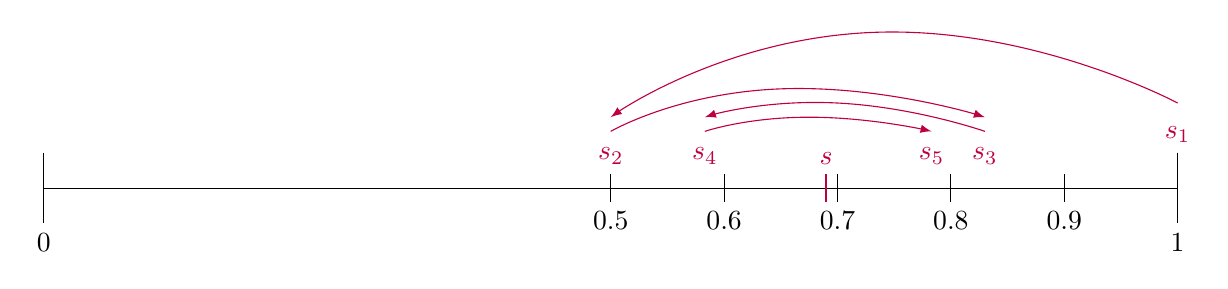
\begin{tikzpicture}[scale=.9]
\draw (0,0) -- (16,0);
\foreach \x in {0,1}{
	\draw (\x*16, 0.5) -- (\x*16,-0.5) node[below]{$\x$};
}
\foreach \x in {0.5,0.6,0.7,0.8,0.9}{
	\draw (\x*16, 0.2) -- (\x*16,-0.2) node[below]{$\x$};
}

\node[above, purple] at (16,0.5) {$s_1$};
\node[above, purple] at (0.5*16,0.2) {$s_2$};
\node[above, purple] at (0.83*16,0.2) {$s_3$};
\node[above, purple] at (0.583*16,0.2) {$s_4$};
\node[above, purple] at (0.783*16,0.2) {$s_5$};

\node[above, purple] at (0.69*16,0.2) {$s$};
\draw[purple, thick] (0.69*16, 0.2) -- (0.69*16,-0.2);

\draw [-latex, purple] plot[smooth, tension=1] coordinates {(16,1.2) (11.8,2.2) (8,1)};
\draw [-latex, purple] plot[smooth, tension=1] coordinates {(8,0.8) (10.4,1.4) (0.83*16,1)};
\draw [-latex, purple] plot[smooth, tension=1] coordinates {(0.83*16,0.8) (11.2,1.2) (0.583*16,1)};
\draw [-latex, purple] plot[smooth, tension=1] coordinates {(0.583*16,0.8) (10.8,1) (0.783*16,0.8)};
\end{tikzpicture}\\
Man kann zeigen: $s=\ln 2 = 0,6931$
\item \emph{Verleichskriterien für Reihen mit nicht-negativen Gliedern}
\paragraph{Satz 8:} (Majoranten-Kriterium)\\
Seien $(a_n)_{n\geq n_0}, (b_n)_{n\geq n_0}$ Folgen mit $0 \leq a_n \leq b_n$ für alle $n\geq n_1 \geq n_0$ und $\sum_{n=n_0}^\infty b_n < \infty$ (d.h. konvergent). \\
Dann $\sum_{n=n_0}^\infty a_n < \infty$ (d.h. konvergent).

Die Reihe $\sum _{n=n_0}^\infty b_n$ heißt dann konvergente Majorante zur Reihe $\sum_{n=n_0}^\infty a_n$.\\
Beweisidee: $0\leq a_n \leq b_n \rightsquigarrow 0 \leq \sum _{n=n_0}^\infty a_n \leq \sum _{n=n_0}^\infty b_n \leq \infty $
\paragraph{Satz 9:} (Minoranten-Kriterium)\\
Seien $(a_n)_{n\geq n_0}, (b_n)_{n\geq n_0}$ Folgen mit $0 \leq b_n \leq a_n$ für $n\geq n_1 \geq n_0$ und $\sum_{n=n_0}^\infty b_n = \infty$ (d.h. divergent)\\
Dann $\sum_{n=n_0}^\infty a_n = \infty$ (also auch divergent)\\
Die Reihe $\sum_{n=n_0}^\infty b_n$ heißt divergente Minorante der Reihe $\sum_{n=n_0}^\infty a_n$.\bigskip\\
Eine nützliche Vergleichsreihe für die Anwendung der Sätze 8 und 9 ist:\\
$\boxed{\sum_{n=1}^\infty \frac{1}{n^\lambda}= \begin{cases}
\text{konvergent} & \text{für }\lambda > 1\\
\text{divergent} & \text{für }\lambda \leq 1
\end{cases}}$
\subparagraph{Bsp. 10:} Man untersuche das Konvergenzverhalten der folgenden Reihe:
\begin{enumerate}[label=\alph*.)]
\item $\sum_{n=1}^\infty \underbrace{\frac{1}{n^2-n+1}}_{a_n}$ (Vermutung: Verhalten wie $\sum \frac{1}{n^2}$ wegen der Dominanz der höchsten Potenz)\\
Wir versuchen eine konvergente Majorante zu finden.\\
$a_n=\frac{1}{n^2-n+1}\geq \frac{1}{n^2-\frac{n^2}{2}}$ (wegen $n\geq \frac{n^2}{2}$ für $n\geq 2$)\\
Somit $\frac{1}{n^2-\frac{n^2}{2}}= \frac{2}{n^2}=:b_n$\\
Mit der Vergleichsreihe gilt: $\sum_{n=1}^\infty b_n = 2 \sum_{n=1}^\infty \frac{1}{n^2}$ ist konvergent.\\
$\overset{\text{Satz 8}}{\Longrightarrow} \sum_{n=0}^\infty a_n$ ist konvergent, sogar absolut konvergent, da $a_n\geq 0 \; (n \in \mathbb{N})$
\item $\sum_{n=1}^\infty \frac{n^2+4}{n^3+n^2+31}$ (Vermutung: divergent, da Verhalten wie $\sum \frac{n^2}{n^3}=\sum \frac{1}{n}$)\\
Wir versuchen divergente Minoranten zu finden.\\
$a_n = \frac{n^2+4}{n^3+n^2+31}\geq ... \geq \frac{1}{3n}=: b_n$ (für $n\geq 4$)\\
Wieder gilt mit der Vergleichsreihe: $\sum b_n$ divergent. Also folgt mit Satz 9: $\sum_{n=1}^\infty a_n$ divergent.
\end{enumerate}
\item \emph{Quotienten- und Wurzelkritierien}
\paragraph{Satz 10:} (Quotientenkriterium)\\
Sei $(a_n)_{n\geq n_0}$ eine Folge, so gilt:\\
$\boxed{\lim_{n\to\infty}\left|\frac{a_{n+1}}{a_n}\right|\begin{cases}
<1\\
>1
\end{cases}\Rightarrow \sum_{n=n_0}^\infty a_n \text{ ist}\begin{cases}
\text{absolut konvergent}\\
\text{divergent}
\end{cases}}$
\paragraph{Satz 11:} (Wurzelkriterium)\\
Sei $(a_n)_{n\geq n_0}$ eine Folge, so gilt:\\
$\boxed{\lim_{n\to\infty} \sqrt[n]{|a_n|} \begin{cases}
<1\\
>1
\end{cases}\Rightarrow \sum_{n=n_0}^\infty a_n \text{ ist}\begin{cases}
\text{absolut konvergent}\\
\text{divergent}
\end{cases}}$
\subparagraph{Bemerkung:} Falls in Satz 10 oder 11 $\lim ... =1$ gilt, so ist mit diesem Kriterium keine Konvergenzaussage möglich.

\subparagraph{Bsp. 11:}
\begin{enumerate}[label=\alph*.)]
\item $\sum_{n=2}^\infty \underbrace{\left( \frac{1}{\ln(n)}\right)^n \cdot (-1)^n}_{a_n}$\\
Wegen $\sqrt[n]{|a_n|}=\frac{1}{\ln n} \overset{n\to\infty}{\longrightarrow} 0 $ liefert das Wurzelkriterium, dass die Reihe absolut konvergent ist.
\item $\sum_{n=1}^\infty \frac{(-1)^n (2n)!}{(n!)^2}$\\
Wegen $\left|\frac{a_{n+1}}{a_n}\right|=\frac{\frac{(2(n+1))!}{((n+1)!)^2}}{\frac{(2n)!}{(n!)^2}}=\frac{(2n+2)!}{((n+1)!)^2}\cdot \frac{(n!)^2}{(2n)!}=\frac{(2n+2)(2n+1)(n!)^2}{(n+1)^2 (n!)^2}=\frac{(2n+2)(2n+1)}{(n+1)^2}
=\frac{4n^2+4n+2n+2}{n^2+2n+1}\overset{n\to\infty}{\longrightarrow} 4$\\
Daher ist die Reihe divergent.
\end{enumerate}
\end{enumerate}
\end{enumerate}

\subsubsection{Rechenregeln}
\begin{itemize}
\item $\sum_{n=n_0}^\infty a_n$ und $\sum_{n=n_0}^\infty$ konvergent mit Summe $a$ und $b$, dann gilt: 
\begin{itemize}
\item $\sum_{n=n_0}^\infty (a_n+b_n)= a + b$
\item $\sum_{n=n_0}^\infty c\cdot a_n= c\cdot a$
\end{itemize}
\item $\sum_{n=n_0}^\infty a_n$ absolut konvergent $\Leftrightarrow$ die Glieder $a_n$ lassen sich beliebig umordnen, ohne dass sich die Summe ändert.
\item $\sum_{n=n_0}^\infty a_n$ und $\sum_{n=n_0}^\infty b_n$ absolut konvergen mit Summen $a$ und $b$, dann gilt:
\begin{itemize}
\item $\left(\sum_{i=0}^\infty a_i\right)\cdot \left( \sum_{j=0}^\infty b_j\right)=\sum_{i=0}^\infty  \sum_{j=0}^\infty a_i b_j=a\cdot b \qquad \left( =\sum_{n=0}^\infty  \sum_{i=0}^\infty a_i b_{n-i} \quad \text{Cauchy-Produkt}\right)$
\end{itemize}
\end{itemize}